\subsection{实验}
\label{sec:task4-experiments}

\subsubsection{数据预处理与划分}
实验使用课程任务提供的 Thyroid 脱敏数据，共 3,772 条记录，每条记录包含六个连续特征。训练集包含 1,839 个正常样本，测试集包含 1,839 个正常样本和 94 个患病样本，患病比例为 4.86\%。表~\ref{tab:task4-data} 展示了数据划分及类别构成。

\begin{table}[!htbp]
  \centering
  \caption{Thyroid 数据划分与类别构成}
  \label{tab:task4-data}
  \begin{tabular}{lccc}
    \toprule
    集合 & 正常 & 患病 & 合计 \\
    \midrule
    训练集 & 1,839 & 0 & 1,839 \\
    测试集 & 1,839 & 94 & 1,933 \\
    合计 & 3,678 & 94 & 3,772 \\
    \bottomrule
  \end{tabular}
\end{table}

数据特征均为有限数值。选取第 2、3、4 和 6 个特征组成四维输入，使用训练集的均值与标准差完成标准化。实验沿用任务给定的划分和原始记录，测试集中有 56 条正常记录的完整六维特征与训练记录相同。

图~\ref{fig:task4-features} 展示的是正常与患病样本在六个特征上的经验累积分布。患病样本的第 2 个特征向较大取值偏移，第 3、4 和 6 个特征则集中于较低取值区间。选定的四个特征据此描述两类样本的分布差异。


\subsubsection{实验配置与拟合流程}
三个检测器均使用 PyOD 实现~\cite{zhao2019pyod}，在正常训练样本上分别拟合。表~\ref{tab:task4-config} 展示了检测器与融合配置。Isolation Forest 每棵树抽取两个特征，深度上限为 $\lceil\log_2 256\rceil=8$。MCD 的原始支持子集大小为 $\lceil(N+d+1)/2\rceil=922$，拟合时执行校正与重加权，随机状态采用库默认设置。

HBOS 对范围外的取值采用边界延拓。若取值与边界的距离不超过边缘区间宽度的 $\eta$ 倍，则使用边缘区间密度，否则采用该维度的最小区间密度。三个检测器的 \texttt{contamination} 参数用于内部阈值计算。Isolation Forest 输出评分在式~\eqref{eq:task4-iforest} 的基础上增加常数偏移，所得平均秩相同。

\begin{table}[!htbp]
  \centering
  \caption{检测器与融合配置}
  \label{tab:task4-config}
  \setlength{\tabcolsep}{4pt}
  \begin{tabular}{lcc}
    \toprule
    模块 & 参数 & 取值 \\
    \midrule
    Isolation Forest & 树数 / 子样本数 & 1,000 / 256 \\
    Isolation Forest & 特征比例 / 种子 & 0.5 / 42 \\
    HBOS & 区间数 & 10 \\
    HBOS & $\alpha$ / $\eta$ & 0.1 / 0.5 \\
    MCD & 原始支持样本数 & 922 \\
    全部分支 & \texttt{contamination} & 0.05 \\
    秩融合 & 分支数 / 权重 & 3 / $1/3$ \\
    \bottomrule
  \end{tabular}
\end{table}

\begin{figure*}[p]
  \centering
  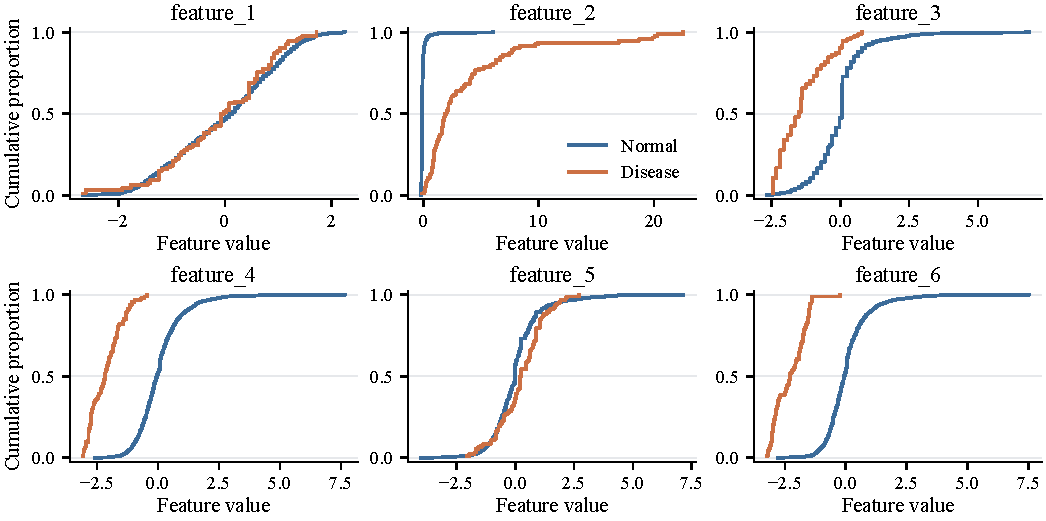
\includegraphics[width=\textwidth]{figures/feature-distributions.pdf}
  \Description{六个特征在测试集正常和患病样本中的经验累积分布，蓝色表示正常，橙色表示患病。}
  \caption{测试集正常与患病样本的特征分布}
  \label{fig:task4-features}

  \par\medskip
  \begin{minipage}{\textwidth}
  \centering
  \captionof{table}{独立检测分支与秩融合方法的测试集结果}
  \label{tab:task4-results}
  \begin{tabular}{lccccc}
    \toprule
    方法 & AUROC & AUPRC & F1 & Precision & Recall \\
    \midrule
    Isolation Forest & \textbf{0.9848} & 0.8932 & 0.8632 & 0.8542 & \textbf{0.8723} \\
    HBOS & 0.9821 & 0.8592 & 0.8187 & 0.7980 & 0.8404 \\
    MCD & 0.9791 & 0.8245 & 0.7923 & 0.7257 & \textbf{0.8723} \\
    秩融合 & 0.9846 & \textbf{0.9060} & \textbf{0.8663} & \textbf{0.8710} & 0.8617 \\
    \bottomrule
  \end{tabular}
  \par\smallskip
  {\small 粗体表示每列最优值，F1、Precision 和 Recall 对应各方法的测试集最佳 F1 阈值}
\end{minipage}

  \par\medskip
  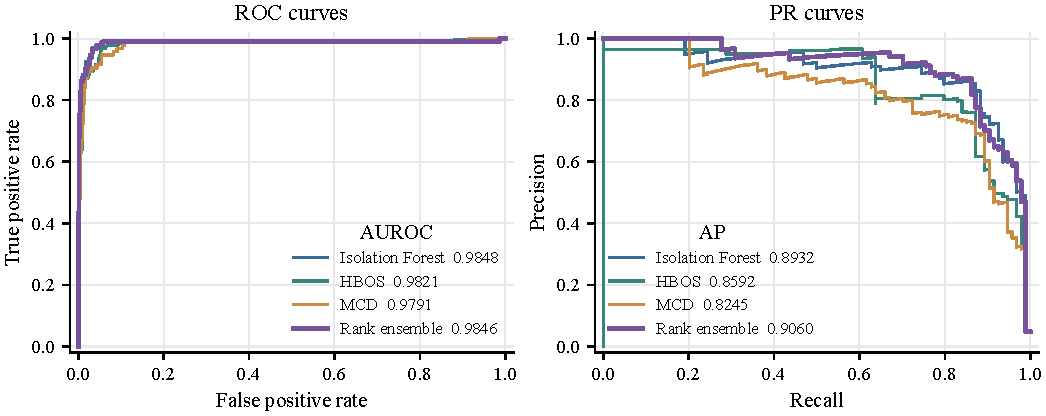
\includegraphics[width=\textwidth]{figures/roc-pr-curves.pdf}
  \Description{左图比较四种方法的 ROC 曲线，右图比较精确率召回率曲线，图例给出相应 AUROC 与 AP。}
  \caption{独立检测分支与秩融合方法的 ROC 和 PR 曲线}
  \label{fig:task4-curves}
\end{figure*}

特征子集和检测器组合依据测试集上的分布分析与评价结果确定。测试标签用于方案选择、指标计算和阈值选择，最终阈值取测试集 F1 最大的候选值
\begin{equation}
  \tau^*=\underset{\tau\in\mathcal T_{\mathrm{te}}}{\arg\max}
  F_1(\tau),
  \label{eq:task4-threshold-selection}
\end{equation}
其中 $\mathcal T_{\mathrm{te}}$ 为测试分数中的不同取值。各独立分支同样采用自身评分上的最佳 F1 阈值。

\subsubsection{评价指标}
评价将患病样本作为正类。为同时描述完整排序和二元判断，报告 AUROC、AUPRC、F1、精确率与召回率。

AUROC 衡量随机抽取的患病样本排在正常样本之前的比例。设正类和负类索引集合分别为 $\mathcal P$ 与 $\mathcal N$，样本数为 $n_+$ 与 $n_-$，则
\begin{equation}
\begin{aligned}
  \mathrm{AUROC}
  =\frac{1}{n_+n_-}\sum_{i\in\mathcal P}\sum_{j\in\mathcal N}
  \Bigl[&\mathbb I(S_i>S_j)\\
  &+\tfrac12\mathbb I(S_i=S_j)\Bigr].
\end{aligned}
\label{eq:task4-auroc}
\end{equation}
ROC 曲线以假阳性率为横轴、真阳性率为纵轴，展示阈值变化时的类别区分情况。

AUPRC 使用平均精确率（Average Precision，AP）计算~\cite{sklearn2026ap}。按阈值降低、召回率递增的顺序，记第 $\ell$ 个工作点的精确率和召回率为 $P_\ell$ 与 $R_\ell$，则
\begin{equation}
  \mathrm{AUPRC}=\mathrm{AP}
  =\sum_{\ell}(R_\ell-R_{\ell-1})P_\ell,
  \label{eq:task4-ap}
\end{equation}
其中初始召回率取 $R_0=0$。该指标根据召回率增量对精确率加权，反映患病样本在高分排序中的集中程度。

在给定阈值下，记真正例、假正例和假负例数分别为 $\mathrm{TP}$、$\mathrm{FP}$ 和 $\mathrm{FN}$。精确率、召回率和 F1 定义为
\begin{equation}
\begin{aligned}
  \mathrm{Precision}&=\frac{\mathrm{TP}}{\mathrm{TP}+\mathrm{FP}},\\
  \mathrm{Recall}&=\frac{\mathrm{TP}}{\mathrm{TP}+\mathrm{FN}},\\
  F_1&=\frac{2\,\mathrm{Precision}\,\mathrm{Recall}}
                 {\mathrm{Precision}+\mathrm{Recall}}.
\end{aligned}
\label{eq:task4-classification-metrics}
\end{equation}
精确率描述判为患病的样本中实际患病者的比例，召回率描述全部患病样本中被识别的比例，F1 汇总这两个方面。


\subsubsection{实验结果与分析}
表~\ref{tab:task4-results} 展示了三个独立检测分支与秩融合方法的测试集结果。融合方法的 AUROC 为 0.9846，AUPRC 为 0.9060。相较 Isolation Forest，融合后的 AUPRC 提高 0.0128，F1 从 0.8632 提高至 0.8663，精确率从 0.8542 提高至 0.8710。

图~\ref{fig:task4-curves} 展示的是各方法的 ROC 曲线与精确率--召回率曲线。四种方法的 ROC 曲线集中于左上区域，反映了正常与患病样本的排序差异。PR 曲线进一步展示了阈值变化时患病样本的检出比例及对应精确率，融合方法的曲线综合了三个分支的排序信息。

\begin{figure}[!htbp]
  \noindent 图~\ref{fig:task4-score-distribution} 展示的是正常与患病样本的融合分数分布。两类样本的分数中位数分别为 0.4472 和 0.9727，患病样本的四分位区间为 $[0.9609,0.9858]$，多数患病记录集中于高分区域。
  \par\medskip
  \centering
  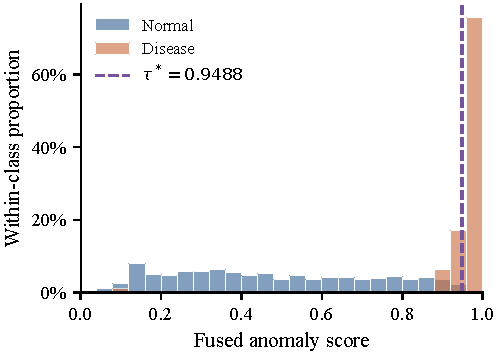
\includegraphics[width=\linewidth]{figures/score-distribution.pdf}
  \Description{正常与患病样本的融合异常分数直方图，各类按样本比例表示，竖线标出测试集最佳 F1 阈值。}
  \caption{正常与患病样本的融合分数分布}
  \label{fig:task4-score-distribution}
\end{figure}

\begin{figure}[!htbp]
  \noindent 图~\ref{fig:task4-confusion} 展示的是测试集最佳 F1 阈值 $\tau^*\approx0.948844$ 下的混淆矩阵。94 个患病样本中识别出 81 个，1,839 个正常样本中正确判断 1,827 个。该阈值下的 F1 为 0.8663，精确率为 0.8710，召回率为 0.8617。
  \par\medskip
  \centering
  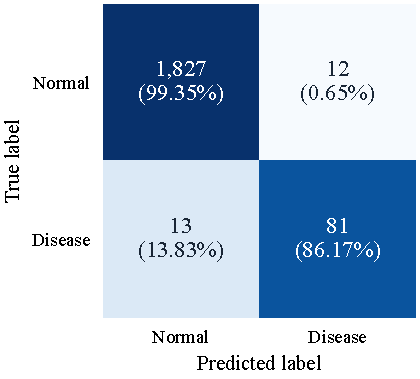
\includegraphics[width=\linewidth]{figures/confusion-matrix.pdf}
  \Description{测试集最佳 F1 阈值下的混淆矩阵，真负例 1827，假正例 12，假负例 13，真正例 81。}
  \caption{测试集最佳 F1 阈值下的混淆矩阵}
  \label{fig:task4-confusion}
\end{figure}
\FloatBarrier
